\documentclass[a4paper, 12p]{article}
\usepackage[spanish]{babel} 
\usepackage{amsmath} 
\usepackage[colorlinks=true]{hyperref}
\usepackage{enumitem} 
\usepackage{graphicx}   
\usepackage[a4paper,top=3cm,bottom=3cm,left=3cm,right=3cm,marginparwidth=1.75cm]{geometry} 
\usepackage[]{subfigure}
\graphicspath{{./graficos/Lab-Termo/Git/Documentos}} 
\usepackage{float}
%\usepackage[]{txfonts}
\usepackage{multicol}



\newenvironment{Figura}
{\par\medskip\noindent\minipage{\linewidth}}
{\endminipage\par\medskip}

%==================================================================================
\begin{document}
\begin{titlepage}
      \begin{center}     
              
            
\includegraphics[width=0.2\textwidth]{img/escudo_udec.png}                       %Para poner logo udec   %{nombre carpeta\nombreimagen}
            
            
            
            \vspace{1cm}
            \textsc{{\LARGE Universidad de Concepción}}
            
            \vspace{1cm}
            {\scshape\Large Facultad de ciencias fisícas y matemáticas \par}
            \vspace{2cm}
            {\scshape\Huge Laboratorio 3 \par}
            \vspace{2cm}
            {\itshape\Large Proyecto laboratorio termodinámica \par}
            \vfill
            {\Large Autores: \par}
            {\Large Martina Contreras, Noemí De La Peña, Benjamín Opazo. \par}
            \vfill
            \vfill
            {\Large Profesor: \par}
            {\Large Claudio Alonso Faúndez Araya \par}
            \vfill
            \vfill
            {\Large Carrera: \par}
            {\Large Ciencias fisícas \par}
            \vfill
            \vfill
            {\Large Ayudante: \par}
            {\Large Renata Hernández Lopez \par}
            \vfill
            {\Large Noviembre 2022 \par}
      \end{center}
\end{titlepage}            
 

\tableofcontents
\newpage

%========Introducción
\section{Introdución}
En este informe se presentarán los datos obtenidos en la experiencia de laboratorio, con el fin de calcular el calor específico de una barra de acero.
Primero se mencionarán los objetivos de este laboratorio, después definiremos que es un calor específico y el Principio de Conservación de la Energía. 
Luego, expondremos los materiales utilizados y el procedimiento a seguir, del cual obtendremos, datos necesarios para responder a las preguntas propuestas en el análisis.
Para finalizar, diremos si se lograron cumplir los objetivos y veracidad de nuestra hipótesis

\section{Objetivos}
\begin{itemize}
      \item Determinar experimentalmente el calor específico de un trozo de metal (alumio, cobre ó acero).
      \item Comparar el valor determinado con los existentes en la literatura.
\end{itemize}



%=========Marco Teórico
\section{Marco Teórico} 

\begin{itemize}
      \item \textbf{Capacidad calorífica: }(a cualquier temperatura) se define como  el limite de C cuando $\varDelta T$ tiende a 0:
      \begin{align}
            C = \frac{d'Q}{dT}           \qquad \left[\frac{J}{K}\right]              
      \end{align}
      donde: \\ \\
      $d'Q = $ Representa un pequeño flujo de calor. \\
      $dT = $ Es el correspondiente al cambio de temperatura. 

      \item \textbf{Calor específico: } Capacidad calorífica por unidad de masa o mol.
      \begin{align}
            c = \frac{C}{n}   \quad \left[\frac{J}{Kilo\cdot molK}\right]  \qquad o  \qquad c = \frac{C}{m} \quad \left[\frac{J}{KgK}\right]
      \end{align}

      \item \textbf{Cantidad total de calor } que fluye en un sistema en cualquier proceso, viene dado por:
      \begin{align}
            Q = \int d'Q &= \int_{T_i}^{T_F} C\cdot dT \\ \nonumber
                         &= \int_{T_i}^{T_F} mc\cdot dT
      \end{align}
      cuando c es constante, obtenemos que:
      \begin{align}
            Q = mc \, \varDelta T
      \end{align}

      \item \textbf{Principio de conservación de la energía}
      \begin{align} \label{p.energia}
            Q_{a,absorbe} &= Q_{x,cede}  \nonumber \\ 
            m_a c_a(T_e - T_{i,a}) &= -m_x c_x (T_e - T_{ix})    
      \end{align}
      donde: \\
      $T_e =$ Temperatura de equilibrio, \\
      $T_i =$ Temperatura inicial, \\
      \textbf{'-'} = Indica que el calor de un cuerpo se cede. \\
      $C_{a,x} =$ Calor específico.

      
\end{itemize} 
Cada concepto fue extraído de \cite{libro}. \\

Nuestra hipótesis es:
\begin{itemize}
      \item Se puede calcular el calor específico de un trozo de metal, usando el principio de conservación de la energía \eqref{p.energia} .
\end{itemize}


%=========Materiales
\section{Materiales}


\begin{itemize}
      \item Generador de vapor PASCO TD-8556A,
      \item Vaso precipitado,
      \item calorímetro,
       \item soporte universal,
      \item termómetros de mercurio x2,
      \item agua,
      \item balanza digital,
      \item trozo de metal.
\end{itemize}



\begin{figure}[H]
    \begin{subfigure}
          \raggedleft
          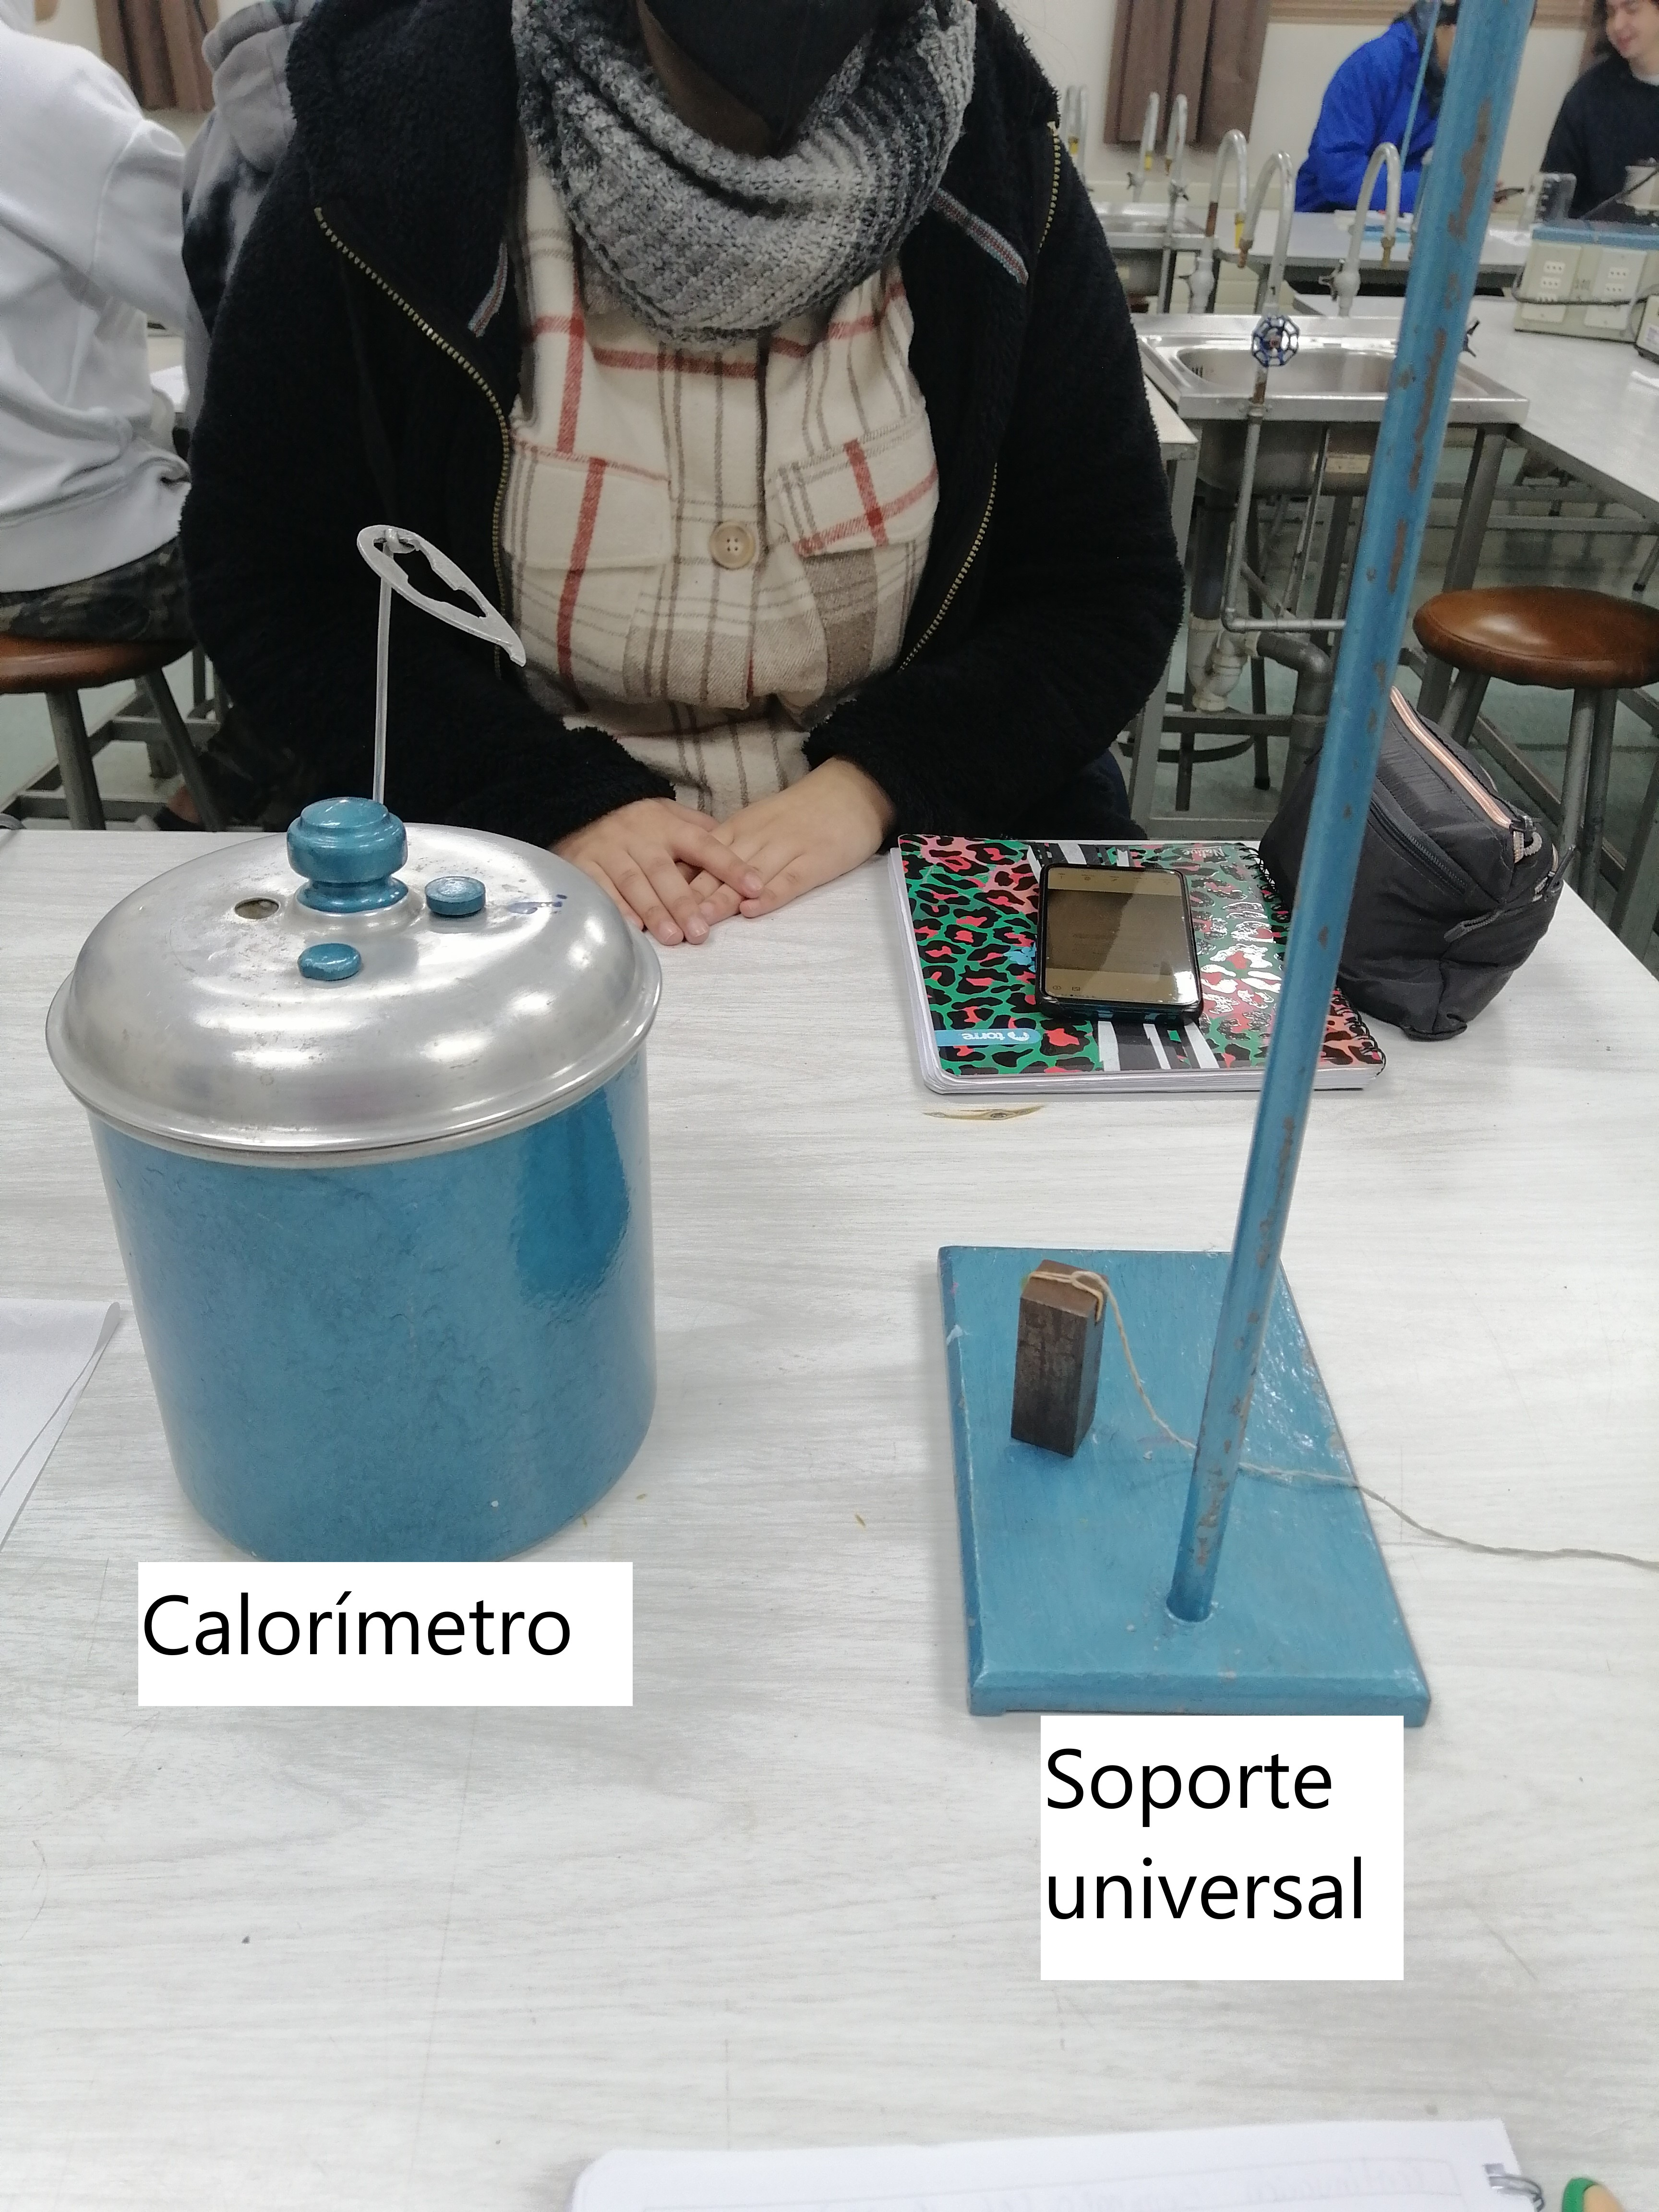
\includegraphics[width=4cm, height=4cm]{img/imag1.jpg}
    \end{subfigure}
    \begin{subfigure}
          \raggedleft
          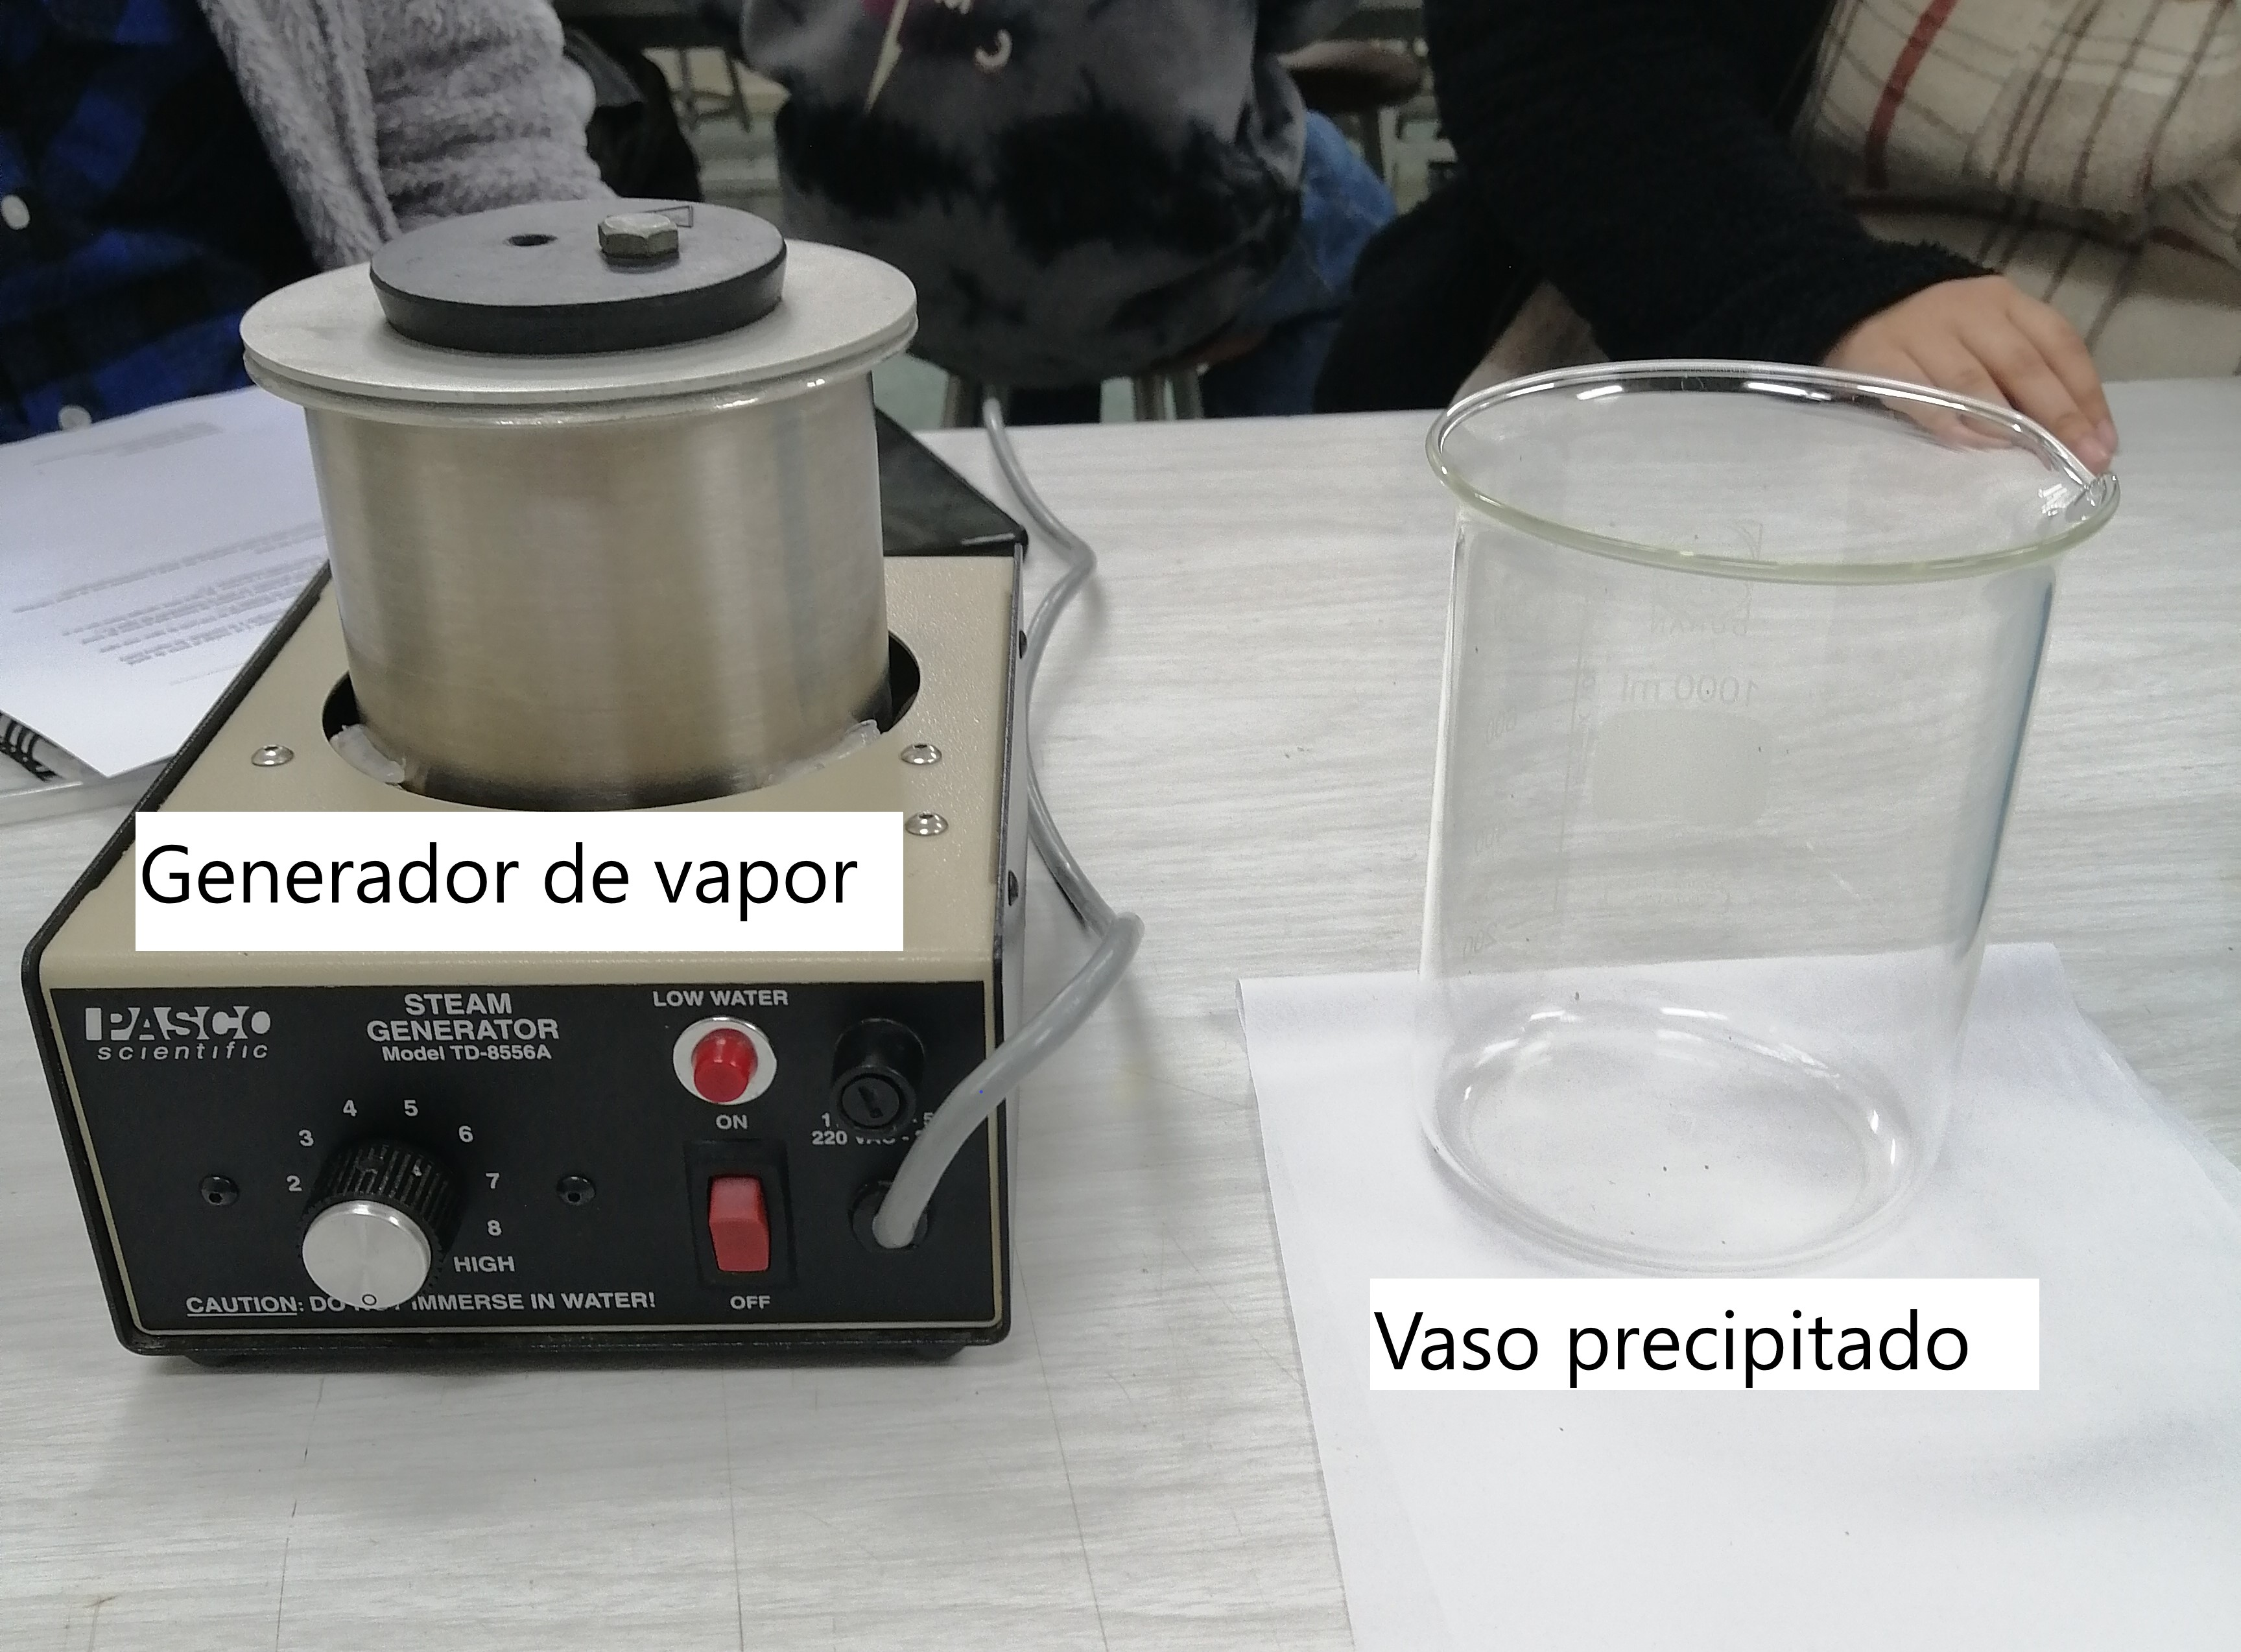
\includegraphics[width=4cm, height=4cm]{img/imag2.jpg}
    \end{subfigure}
    \begin{subfigure}
          \raggedleft
          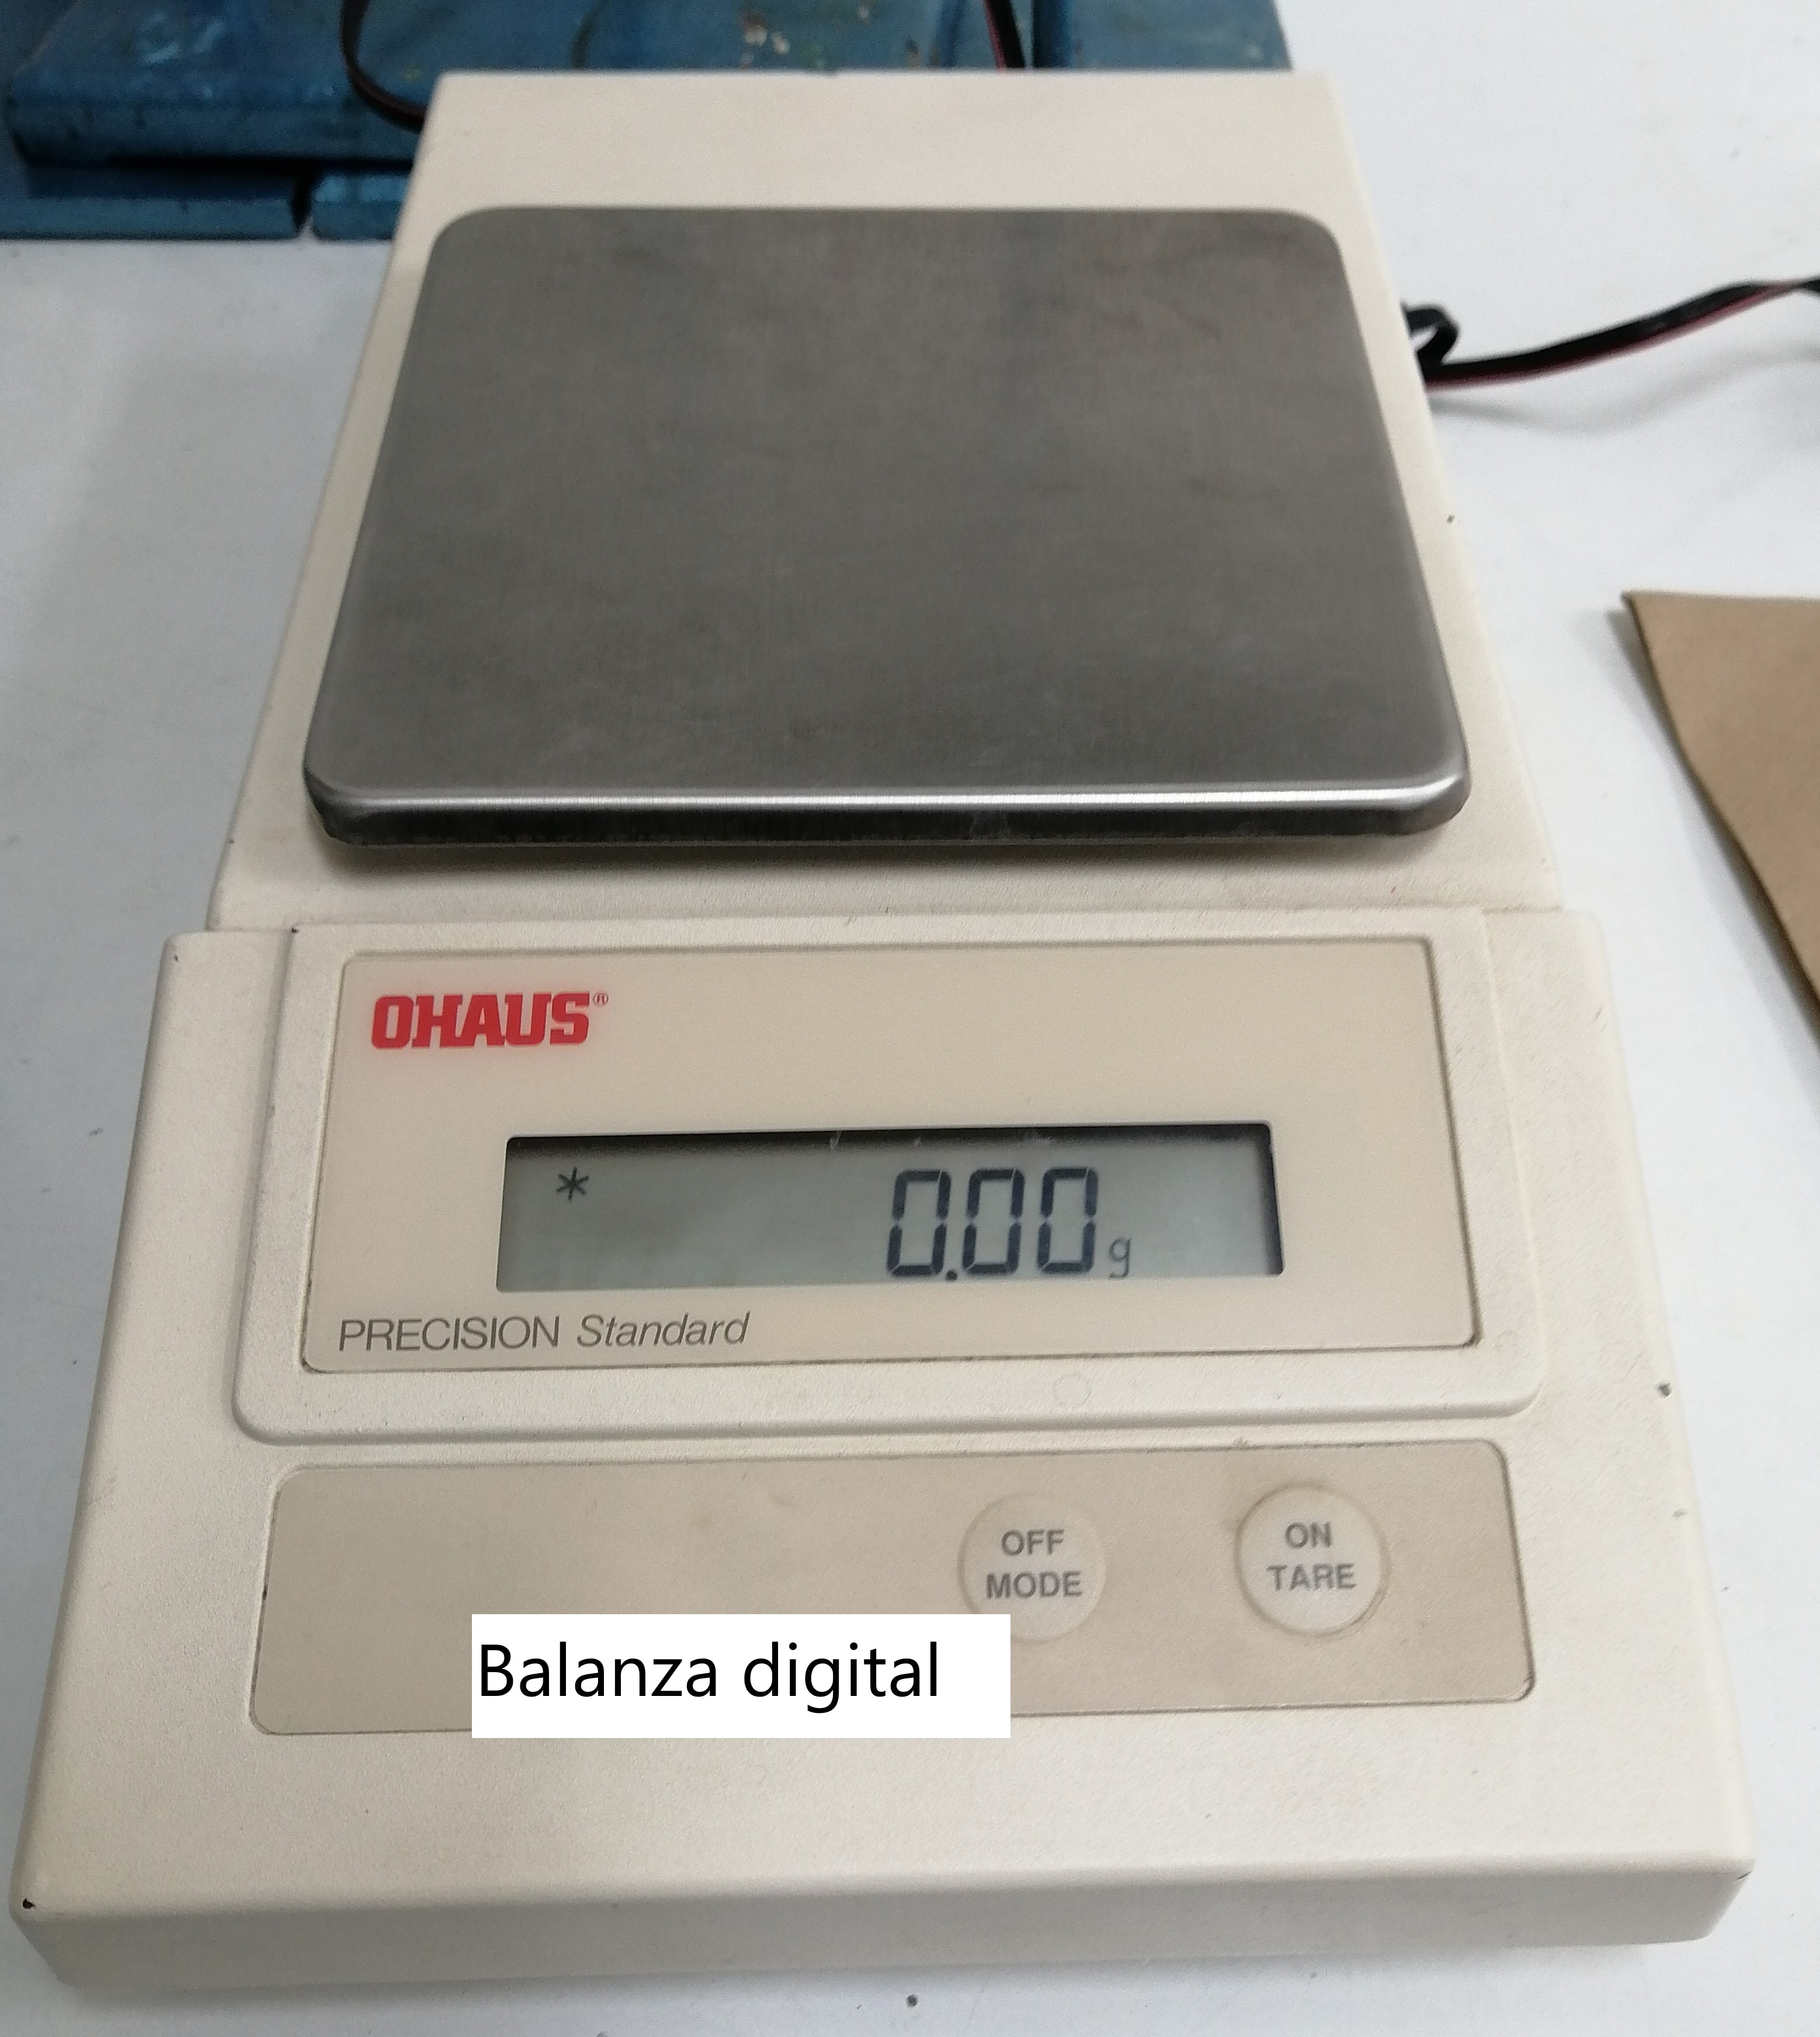
\includegraphics[width=4cm, height=4cm]{img/imag3.jpg}   
    \end{subfigure}   
    \begin{subfigure}
          \raggedleft
          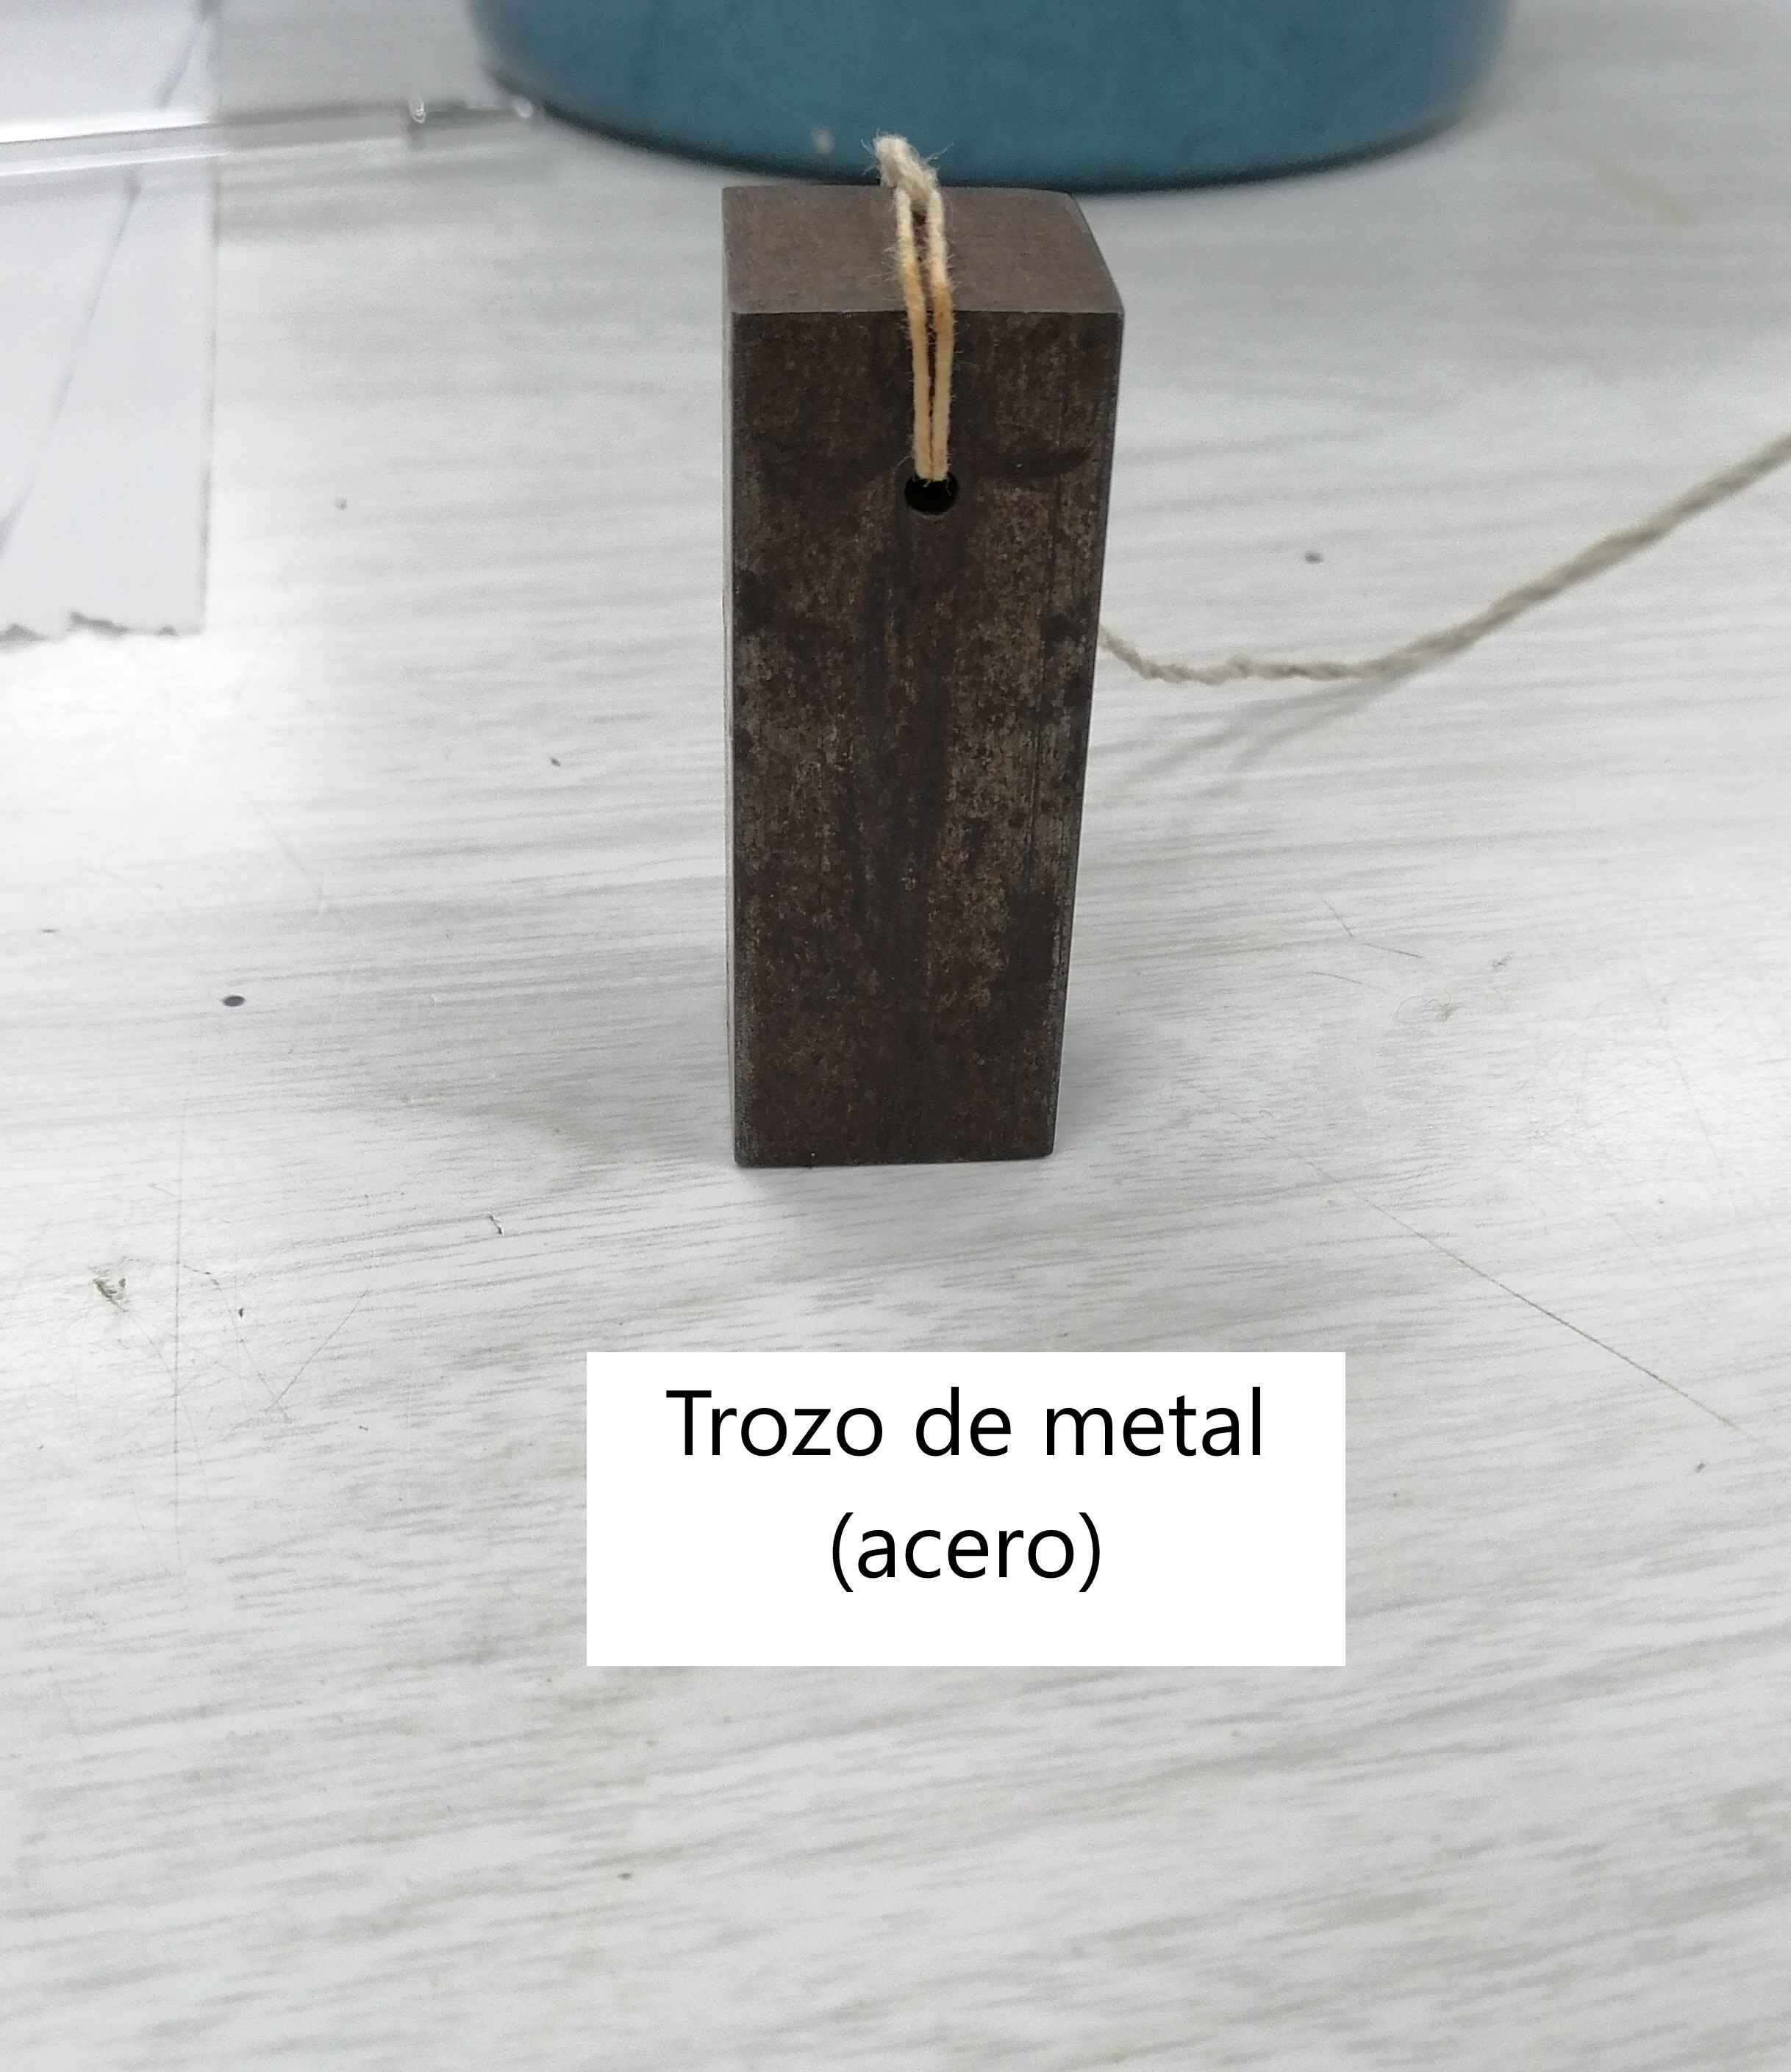
\includegraphics[width=4cm, height=4cm]{img/imag4.jpg} 
    \end{subfigure}
    \begin{subfigure}
          \raggedleft
          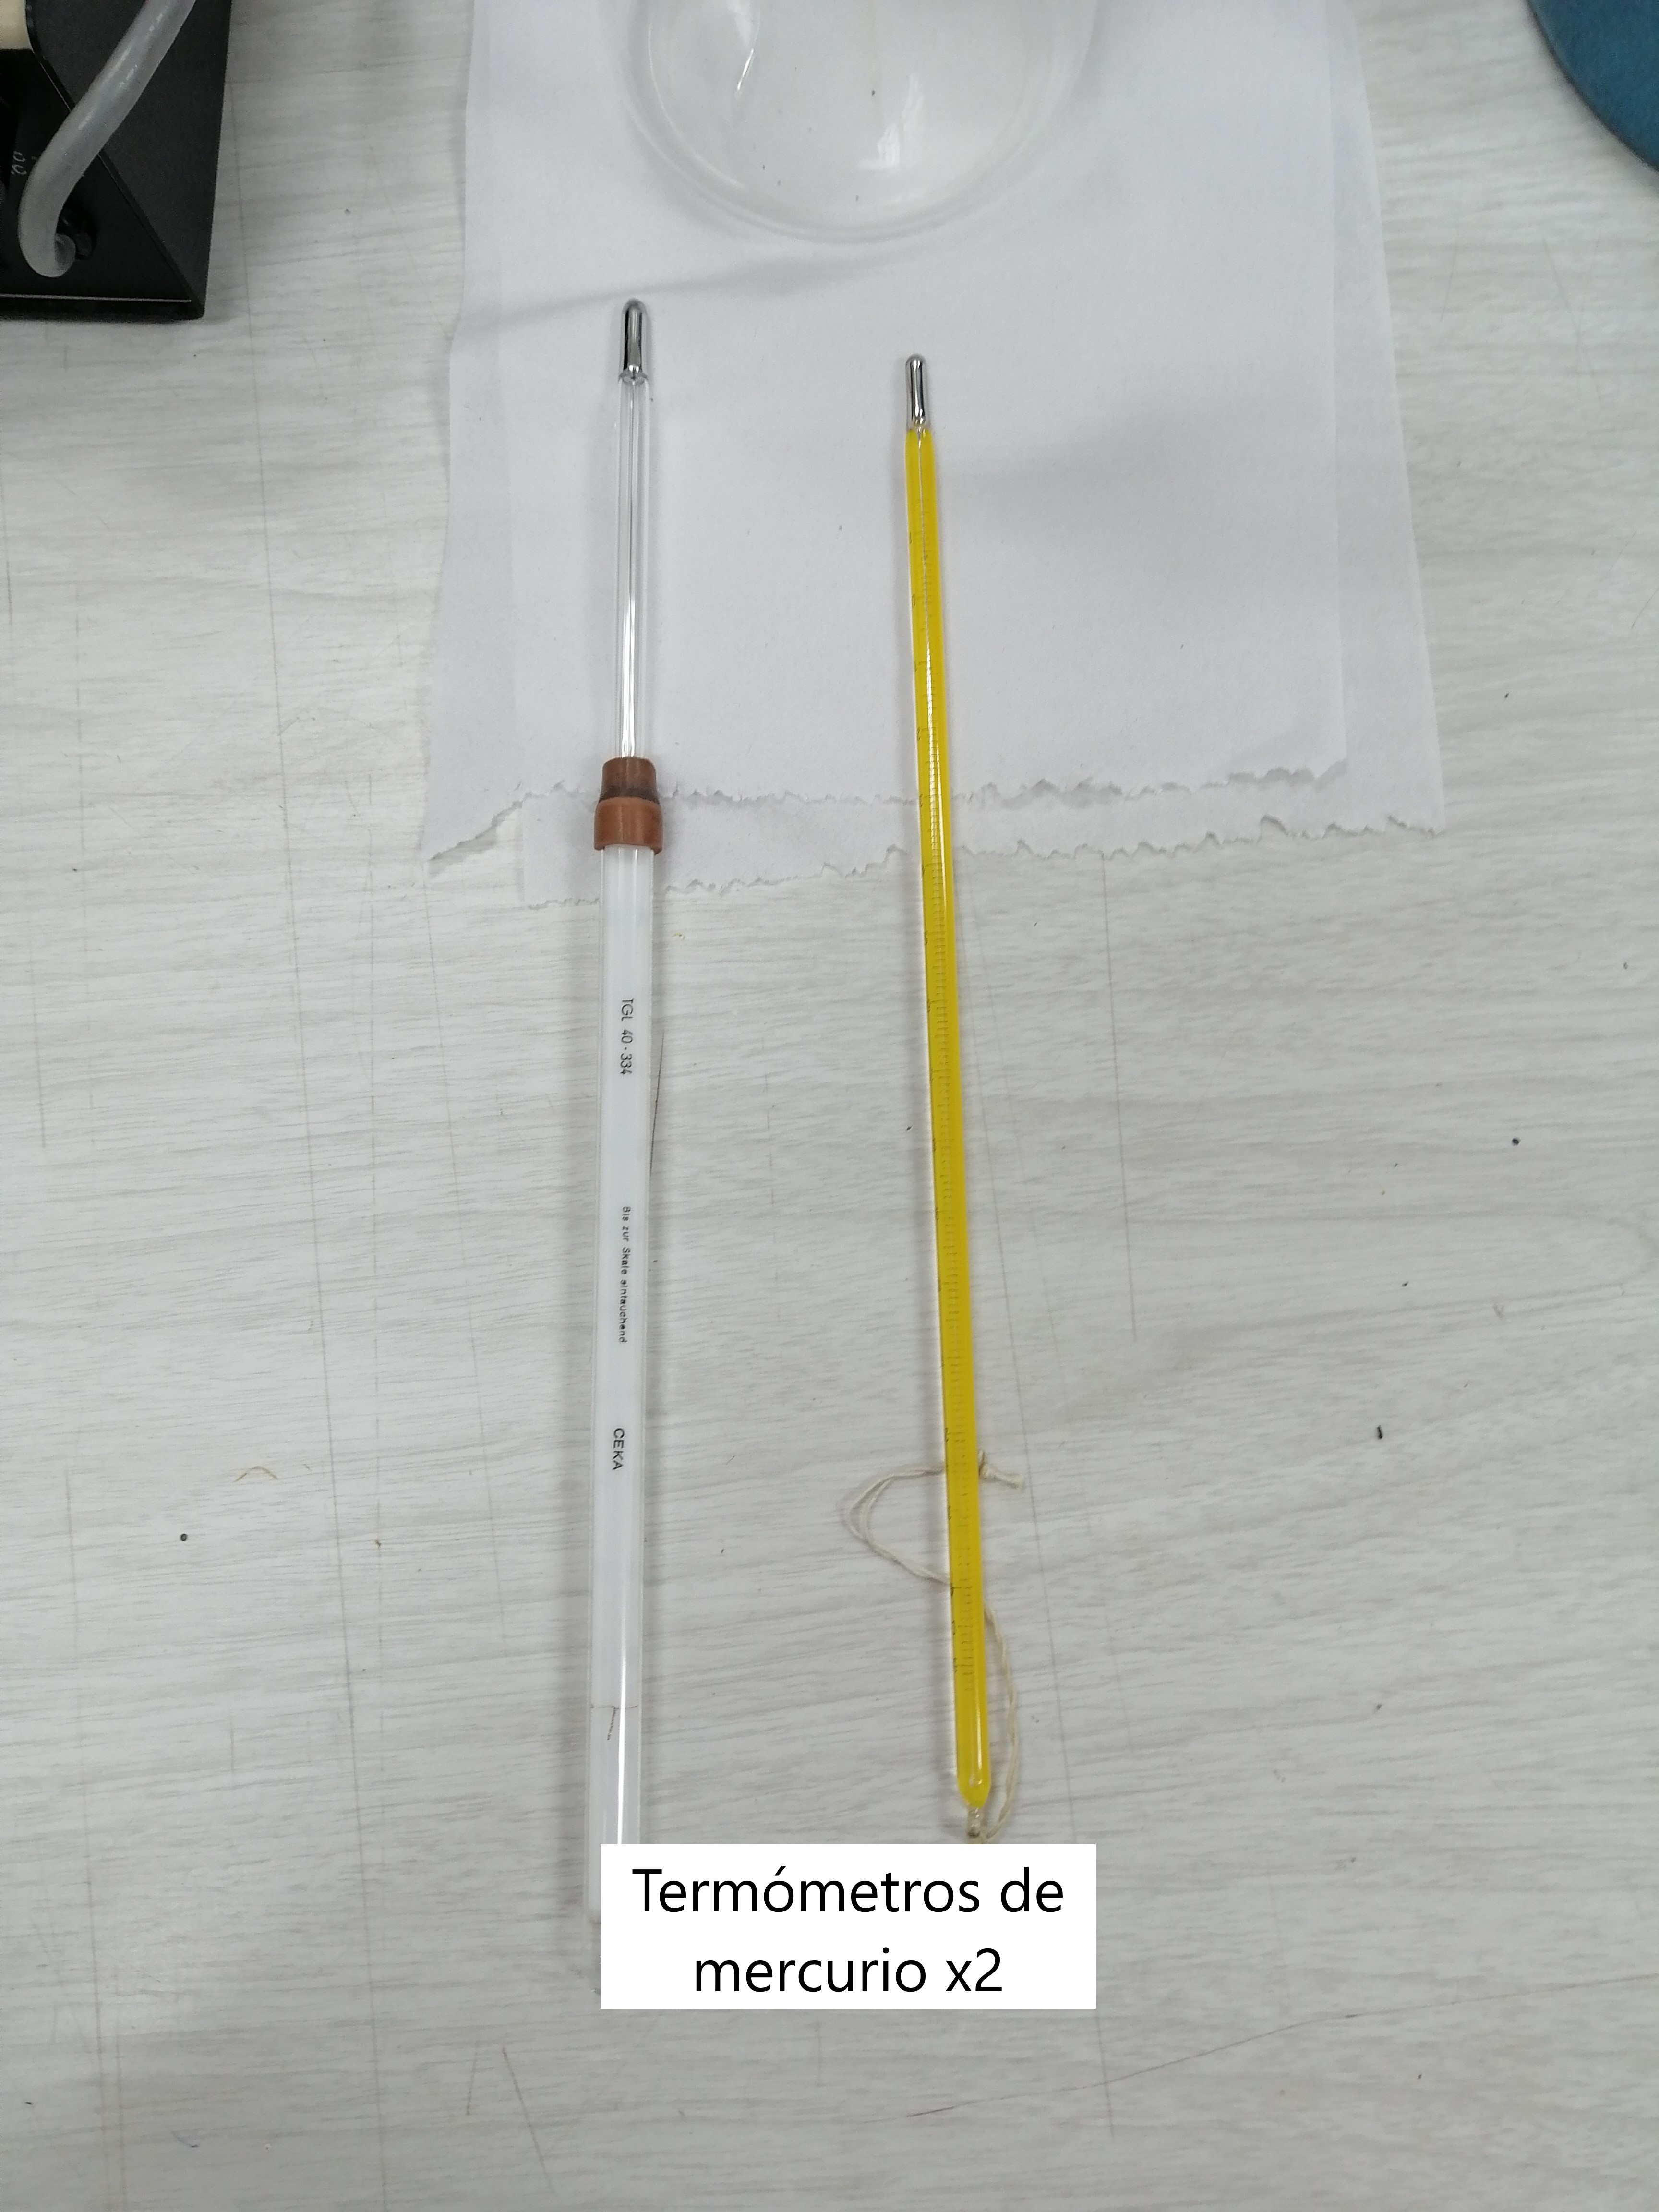
\includegraphics[width=5cm, height=4cm]{img/imag5.jpg} 
    \end{subfigure}
\end{figure}     


\section{Procedimiento}

\begin{itemize}
      \item Primero, masamos el trozo de metal $m_M$.
      \item Luego, vaciamos alrededor de $850 [ml]$ de agua en el generador de vapor, y colgamos el trozo de metal desde el soporte universal,
      de modo que quede totalmente sumergido. Encendemos el aparato y esperamos hasta que el agua hierva.
      \item Paralelamente, masamos $350 [ml]$ de agua, $m_a$, luego calculamos su temperatura, $T_{a,i}$ y la vaciamos en el calorímetro. 
      \item Una vez que hierve el agua, dejamos encendido hasta por 2 minutos, de forma que el trozo de metal alcance el 
      equilibrio térmico con el agua del generador. Después, medimos la temperatura del agua $T_{m,i}$.
      \item Trasladamos el trozo de metal hacía el calorímetro y lo cerramos. Luego, agitamos el agua hasta que en el interior se 
      alcance el equilibrio térmico. Por último, medimos la temperatura final, $T_f$.
\end{itemize}

\section{Análisis}
\begin{enumerate}
      \item Calcular el calor específico (c) del metal.\\
      R: Nuestros datos son:\\ \\
                     $m_{a} = 281.5 g$ ó $0.2815 kg$, masa del agua \\
                     $m_{Ac} = 225.9 g$ ó $0.2259 kg$, masa del acero\\
                     $Ti_a$ = 17ºC ó 290K , temperatura inicial del agua. \\
                     $Ti_Ac$ = 100ºC ó 373K, temperatura inicial del acero. \\ 
                     $c_{a}$ = 4184 J/kgK , calor especifíco del agua. \cite{agua}\\
                     $Tf$ = 23ºC ó 296K, temperatura final.\\ 
                     
                     Primero, como el acero es el que está a mayor temperatura que el agua, el acero será el que ceda calor y el agua la que absorbe calor, y por el principio de conservación de la energía, tenemos que:\\
                     \begin{equation}\label{eq1}
                     Q_{a} = -Q_{Ac},
                     \end{equation}
                     donde $ Q_{a}$ es el flujo de calor del agua, y $Q_{Ac}$ es el flujo del calor del acero.\\ 
                     
                     El flujo de calor del agua viene dado por:
                     \begin{equation}\label{eq2}
                     Q_{a} = \int_{Ti}^{Tf} \! \, d^{\prime}Q  = \int_{Ti}^{Tf} \! m_{a}c_{a} \, dt = c_{a} m_{a} \Delta T,
                     \end{equation}
                     El flujo de calor del acero viene dado por:
                     \begin{equation}\label{eq3}		       
                     Q_{Ac} = \int_{Ti}^{Tf} \! \, d^{\prime}Q  = \int_{Ti}^{Tf} \! m_{Ac}c_{Ac} \, dt = c_{Ac} m_{Ac} \Delta T,
                     \end{equation}
                    
                    Reemplazando \ref{eq2} y \ref{eq3} en \ref{eq1}, tenemos que 
                    \begin{equation}\label{eq4}
                    c_{a} m_{a} \Delta T = -c_{Ac} m_{Ac} \Delta T
                    \end{equation}
                    
                    Reemplazando nuestros datos en \ref{eq4}, tenemos que 
                    \begin{equation}\label{eq5}
                    4184 \dfrac{J}{kgK} \times 0.2815Kg(296K - 290K) = -(c_{Ac} \times 0.2259kg(296K - 373K))
                    \end{equation}
                    
                    Como nosostros queremos calcular $c_{Ac}$, despejamos $c_{Ac}$ en \ref{eq5}, así tenemos que.\\
                    $c_{Ac} = 406.27 \dfrac{J}{kgK}$  		    
                      
      \item Colocar el valor de referencia para el calor específico del metal y comparar con el valor calculado (usando error porcentual).\\
      El valor de referencia será $c_{Ac}$ = 460 J/kgK el cual fue obtenido de \cite{acero} y nuestro valor experimental es  $c_{Ac} = 406.27 J/kgK$, calculado anteriormente,
      luego, usando: \\
      \begin{align*}
            Error &= \left|\frac{valor \, experimental - valor \, teorico}{valor \, teorico} \cdot 100 \right|, \\
      \end{align*}
      finalmente, el error porcentual es:
      \begin{align*}
            Error &= \left|\frac{406.27 \, J/kgK - 460 \, J/kgK }{460 \, J/kgK} \cdot 100 \right| \\
                  &= 11,68\%
      \end{align*}
      
      
    \end{enumerate}   


\section{Conclusión}
Al finalizar este informe, podemos decir que los objetivos se cumplieron. Calculamos el calor específico de la barra de acero y la comparamos con la existente en la literatura.
Además, gracias a los datos obtenidos, logramos demostrar la veracidad de nuestra hipótesis, por la cual, podemos concluir que: \\
Es posible calcular, aproximadamente, el calor específico de un trozo de metal, a través de la ley de la conservación de la energía.




\begin{thebibliography}{6}
      \bibitem{libro} Sears, F. W., Salinger, G. L. \& Peris, A. J. (2021, 10 enero). Termodinámica, teoría cinética y termodinámica estadística (Spanish Edition) (1.a ed.). Reverte.
      \bibitem{profe} Faundez Araya, C. A. (s. f.). Capítulo 3. Primer Principio de la Termodinámica [Diapositivas]. Universidad de Concepción, 2022.
      \bibitem{agua}Fundación Aquae. (2021, 10 agosto). CP del agua: significado y valores - Fundación Aquae. FundaciÃ3n Aquae. 
      \url{https://www.fundacionaquae.org/wiki/cp-del-agua/}
      \bibitem{acero}DeterminaciÃ3n del calor específico de un sÃ3lido. (s. f.). Recuperado 25 de octubre de 2022,
       de \url{http://www.sc.ehu.es/sbweb/fisica/estadistica/otros/calorimetro/calorimetro.htm}
\end{thebibliography}













\end{document}
